\newpage\section{Equipe de Controle}
Considerando o escopo do projeto, o grupo responsável pela parte de controle, associado às informações elaboradas pelos demais grupos apresentará, por meio deste relatório, uma proposta de construção do sistema a partir da utilização de sensores para o monitoramento dos parâmetros: temperatura, pressão, fluxo e nível.\\
Observando as duas propostas apresentadas anteriormente, onde um sensor de temperatura principal seria auxiliado por sensores de temperatura de redundância, tem-se que a proposta definida é semelhante. A diferença está no foco dado à cada sensor em diferentes períodos do teste do foguete híbrido. Durante a realização do teste, os sensores de temperatura internos (localizados no reservatório e na tubulação) serão analisados com maior atenção, a fim de manter a faixa de temperatura no nível de bom funcionamento do sensor de pressão da Kistler. Após o encerramento do teste, o foco principal estará no sensor de temperatura externo (localizado no adaptador da câmara de combustão), já que a transferência de calor que se dá após o teste é alta e deve-se controlar a temperatura do sistema para que os componentes mantenham sua integridade.\\
Diante disso, há no mercado uma gama enorme de sensores que podem ser escolhidos para o funcionamento de um projeto, e a escolha destes deve levar em consideração não só questões operacionais do produto requisitado, mas também uma relação custo-benefício. Além do mais, criticidade do projeto demanda o uso de sub-sistemas redundantes, garantindo maior confiabilidade ao controle do sistema.\\
Portanto, considerando os requisitos necessários para o bom funcionamento do sistema, foram definidos seis sensores, sendo eles três de temperatura, um de pressão, um de fluxo e um de nível, que realizarão o monitoramento dos parâmetros cruciais. Serão utilizados também um microcontrolador, bem como circuitos paralelos de comunicação, amplificação de sinal e alimentação.\\
\section{Desenvolvimento}
O sistema de controle foi baseado em cinco partes, sendo elas: coleta de dados, amplificação de sinais, análise de dados, transferência de dados e controle de resposta.
\subsection{Coleta de Dados}
A parte de coleta de dados será realizada pelos sensores e será a porta de entrada para os dados de monitoramento dos principais parâmetros durante a realização do teste. O sensor de pressão da Kistler estará em funcionamento juntamente com todo o sistema de arrefecimento durante o teste. Sendo assim os principais parâmetros a serem monitorados são temperatura (sensor de pressão da Kistler, tubulação e reservatório), pressão (tubulação), fluxo (tubulação) e nível (reservatório). Portanto, após diversas pesquisas, os modelos mais adequados para cumprirem essas funções foram:
\begin{itemize}
	\item \textbf{Sensor de Temperatura para o adaptador da câmara de combustão}:
	\begin{itemize}
		\item \textbf{ Modelo:} TJ36-CASS-116G-6-CC-XCIB;
		\item \textbf{ Descrição:} Sonda TJ36 com cabo de ligação com isolamento cerâmico de Nextel® e revestimento trançado de Inconel® 600, terminações desencapadas;
		\item \textbf{ Material da Bainha:} sonda em aço inox 304;
		\item \textbf{ Categoria do termopar:} tipo K;
		\item \textbf{ Tipo de Junção:} Aterrada;
		\item \textbf{ Dimensões:}
		\begin{itemize}
			\item  Diâmetro da sonda de 1,59 mm (1/16” pol);
			\item Comprimento de 150 mm (6” pol);
			\item Comprimento do fio de 1,0 m.
		\end{itemize}
		\item \textbf{ Temperatura de operação:} -200 ºC a 899 ºC;
		\item \textbf{ Preço:} R\$382,00.
	\end{itemize}
	
\end{itemize}
\begin{figure}[!htb]                   
	\centering                          
	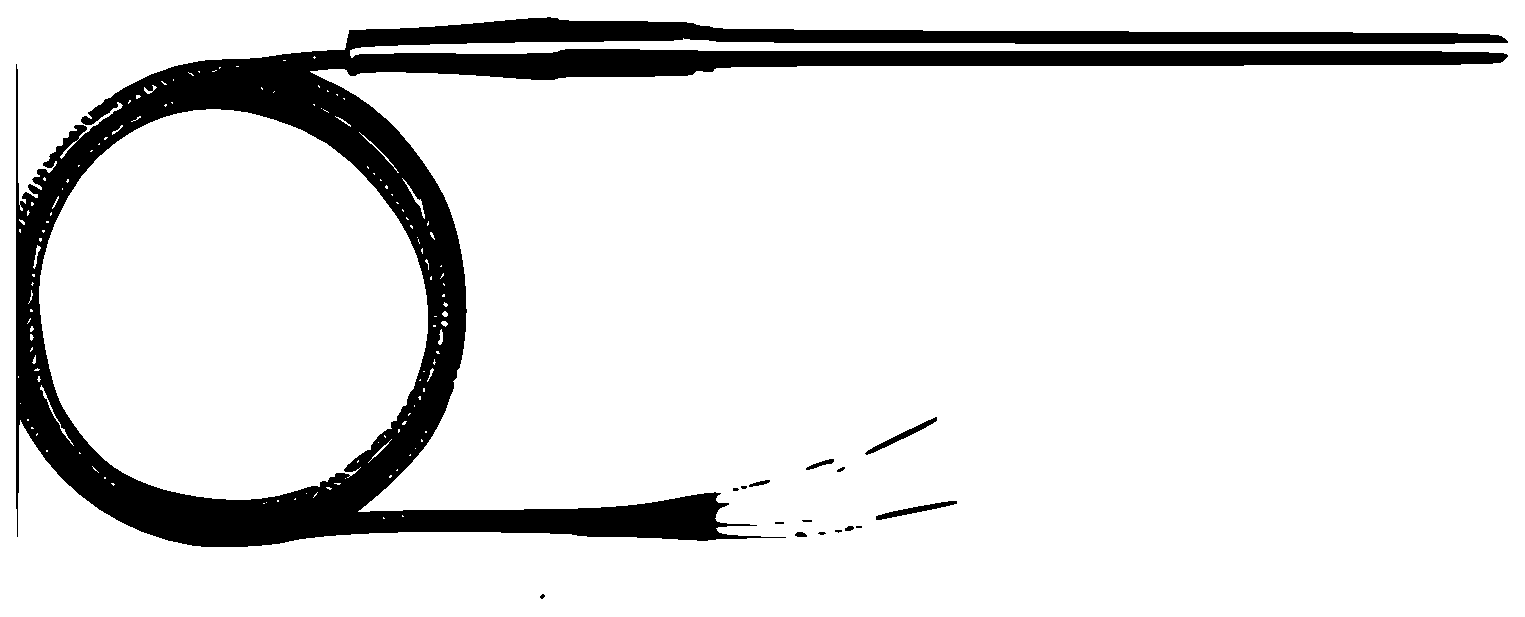
\includegraphics[scale=0.4]{figuras/Sensor1.eps}
	\caption{Sensor de Temperatura para o adaptador da câmara de combustão}               
\end{figure}
\subsection{Explicação:}
	A escolha deste sensor se deve ao fato principalmente da magnitude da temperatura no adaptador que, por meio de simulações realizadas pelo grupo de transmissão de calor, alcança a faixa de até $450^o C$, na posição em que o sensor de pressão principal está localizado. Foi estabelecido um fator de segurança igual a 2, teorizando uma temperatura máxima de $900^{o}C$ no adaptador, o que dá maior margem para erros e falhas. Dessa forma, a escolha de um termopar tipo K se justifica, se for considerado a faixa de medição padrão $(-200^o C a 1250^o C)$ e a alta disponibilidade desse tipo de termopar no mercado.\\
	A junção da bainha é do tipo aterrada, onde os fios do termopar estão em contato físico direto com o interior da parede da sonda. Isso resulta em uma relação resposta/proteção ideal para o caso analisado, já que o material utilizado é o aço, que é conhecidamente um bom condutor térmico. Comparativamente, se fosse utilizada uma junção isolada, o tempo de resposta seria mais demorado, já que entre os fios do termopar e a parede da sonda existe um isolamento que impede o contato direto entre os dois. Já para uma junção exposta o efeito seria o contrário, com um tempo de resposta mais ágil, porém os fios do termopar estariam em maior risco de serem danificados e comprometerem o sensoriamento.\\
	Considerando também o local onde o sensor deverá ser acoplado, as dimensões do produto são apropriadas. Porém, este dimensionamento pode ser melhor adequado à situação requerida através do acessório chamado bucim, peça anelar metálica que pode ser utilizada a fim de permitir o ajuste exato da imersão da sonda no adaptador. Para isso, será necessário o furo de uma rosca na lateral superior, próximo ao encaixe do sensor de pressão da Kistler, local onde a temperatura pode ser medida com maior exatidão. Um modelo CAD feito com o software Catia V5R19 foi desenvolvido a fim de ilustrar o adaptador:
\begin{figure}[!htb]                   
		\centering                          
		
\includegraphics[scale=1]{figuras/adaptador.eps}
		\caption{Adaptador da Câmara de Combustão}               
\end{figure}
\subsection{Tempo de Resposta}
Levando em consideração que os testes realizados no foguete híbrido estão entre 15 e 40 segundos, é necessário que o tempo de resposta dos sensores em geral esteja na escala de milissegundos, a fim de maximizar a coleta de dados e auxiliar na obtenção de resultados dos testes.\\
Segundo o Manual Técnico de Temperatura da empresa OMEGA, o tempo de resposta de um sensor é o tempo necessário para que um sensor responda a uma mudança de valor na temperatura. Também pode ser vista como uma medida de comparação da velocidade em que um sensor indicará uma mudança nas condições de temperatura e, normalmente, é um componente para determinar o tempo de resposta do sistema .\\
Considerando essa definição, a imagem abaixo é a representação gráfica da relação do diâmetro da bainha em polegadas com o tempo de resposta em segundos, de acordo com o tipo de junção da bainha:
\begin{figure}[!htb]                   
	\centering                          
	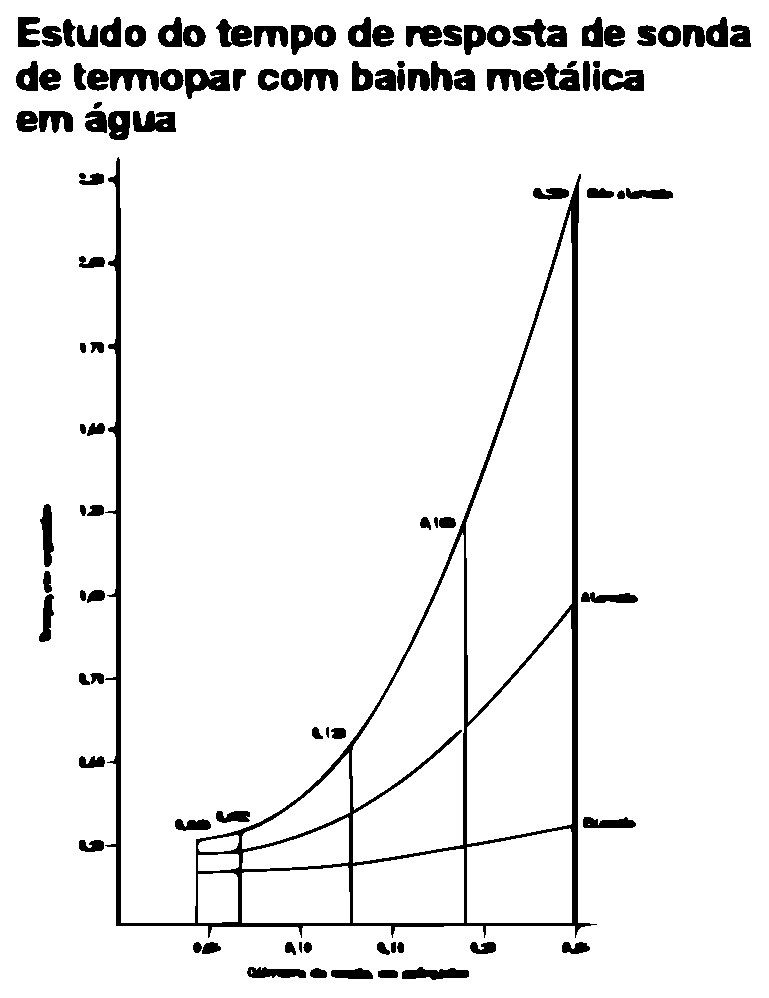
\includegraphics[scale=1]{figuras/Figura3.eps}
	\caption{Estudo do Tempo de Resposta}               
\end{figure}	
\begin{itemize}
	\item \textbf{ Sensor de Temperatura para a tubulação e para o reservatório:}
	\begin{itemize}
		\item \textbf{ Modelo:} Sensor de Temperatura DS18B20;
		\item \textbf{ Descrição:} Sensor de temperatura versão à prova de água do sensor DS18B20; 
		\item \textbf{ Material de composição:}
		\begin{itemize}
			\item \textbf{ Ponteira:} aço inoxidável.
		\end{itemize}
		\item \textbf{ Faixa de temperatura:} de $ -55^oC$ até $+125^oC$;
		\item \textbf{ Precisão:} $\pm0,5^oC$ na faixa de $-10^oC a +85^oC$; 
		\item \textbf{ Alimentação:} 5 VDC;
		\item \textbf{ Tempo de resposta:} menor que 750 ms;
		\item \textbf{ Dimensões:}
		\begin{itemize}
			\item Ponteira com 6 mm de diâmetro por 50 mm de comprimento;
			\item Possui cabo de ligação revestido em PVC de 90 cm;
		\end{itemize}
		\item \textbf{ Comunicação:}
		\begin{itemize}
			\item Possui três fios de interface: Fio Vermelho (VCC), Branco ou Amarelo (DADOS), Preto (GND);
			\item Resolução configurável pelo usuário de 9-bits a 12-bits;
		\end{itemize}
		
		\item \textbf{ Preço:} R\$ 16,80.
\end{itemize}
\end{itemize}
\begin{figure}[!htb]                   
	\centering                          
	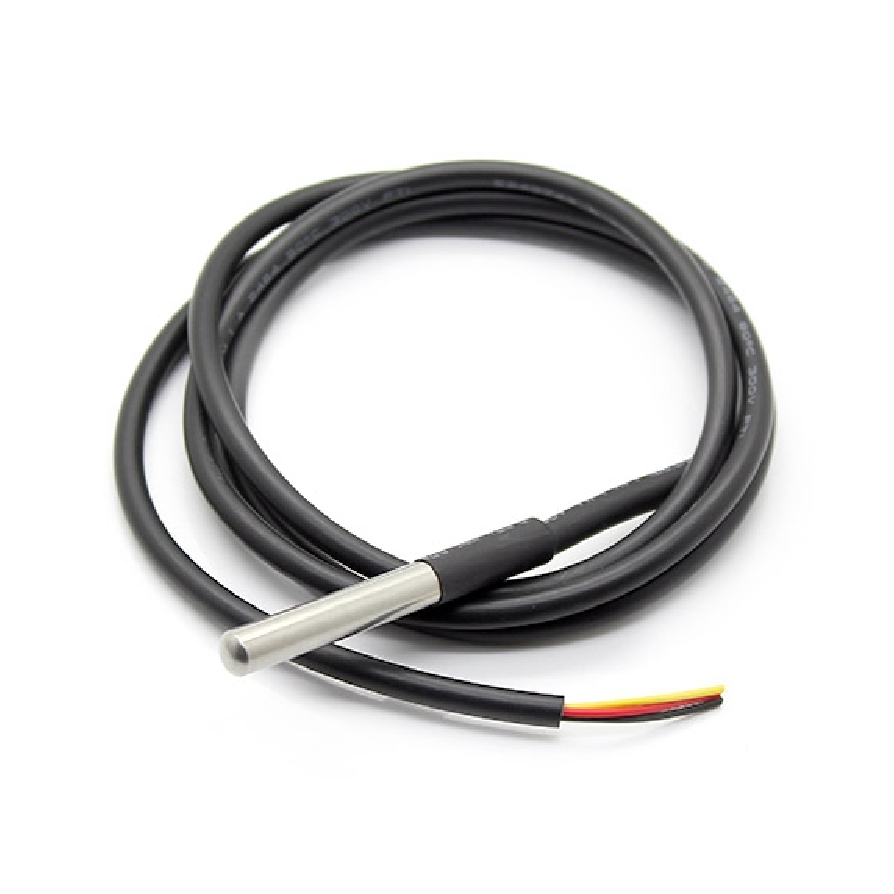
\includegraphics[scale=0.5]{figuras/Figura4.eps}
	\caption{Sensor de Temperatura para a tubulação e para o reservatório}               
\end{figure}
\subsection{Explicação}
Serão utilizados dois sensores deste tipo, um para o reservatório e outro para a tubulação. O sensor que vai no reservatório tem a finalidade de medir a temperatura no local, que segundo estudos do grupo de Transmissão de Calor, deverá estar na faixa de $25 à 30^o$C. A utilização desse sensor é vista como medida de redundância, onde sua principal função é a verificação do funcionamento do sistema de arrefecimento. \\
Já o outro sensor, se encontra próximo a tubulação de saída do sensor de pressão da Kistler, com a finalidade de monitorar a temperatura da água na tubulação. Com as simulações do grupo de Transmissão de Calor foi definido que a temperatura do líquido na tubulação de saída será por volta de $90^oC$. Considerando o local onde o sensor será instalado, será necessário o uso de adaptadores como o bucim, para que possa fixar o sensor na conexão em T adequada. Sendo assim, o uso deste sensor é considerado mais vantajoso, visto que as dimensões do diâmetro e comprimento da bainha especificados (6mm e 30mm, respectivamente) são convenientes para fazer a conexão sem que atrapalhe a medição da temperatura da água na tubulação.\\
Outros fatores cruciais para a escolha desse sensor para essas duas áreas foram a faixa de medição (que é compatível com as duas localidades), o fato do sensor ser à prova d’água e seu tempo de resposta de menos de 750 ms, que geram um ótimo custo-benefício levando em conta que o custo do sensor é mínimo.
\begin{itemize}
	\item \textbf{Sensor de Pressão para a tubulação
	Modelo:} MPX 2200 GP
	\item \textbf{Descrição:} Sensor de Pressão modelo MPX 2200 GP 
	\item \textbf{Tipo de medição:} Tipo Gauge, Pressão de calibre;
	\item \textbf{Pressão de Operação:} 0 a 200 kPa ou 0 a 2 Bar;
	\item \textbf{Temperatura de Operação:} -40 a 125º C;
	\item \textbf{Tempo de resposta:} 1 ms;
	\item \textbf{Tensão de saída:} 40 mV;
	\item \textbf {Alimentação:} 10 a 16 V – 6mA;
	\item \textbf{Sensibilidade:} 0,2 mV/kPa;
	\item \textbf{Dimensões:}
	\begin{itemize}
		\item \textbf{Porta de saída:} Tipo fêmea de 4.62 a 4.93 mm;
	\end{itemize}
	
	\item \textbf{Preço:} R\$ 55,00.
	
\end{itemize}
\begin{figure}[!htb]                   
	\centering                          
	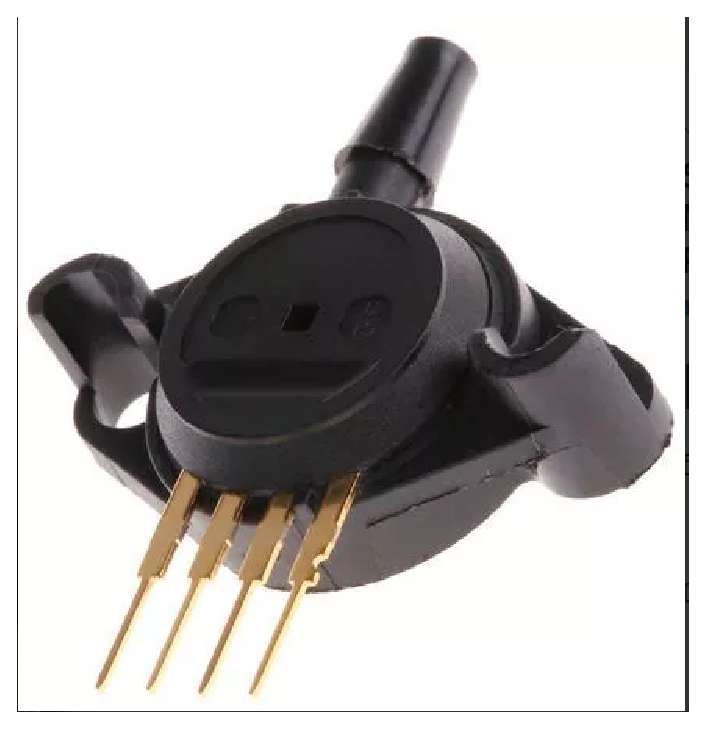
\includegraphics[scale=0.5]{figuras/Figura_5.eps}
	\caption{Sensor de Pressão para a tubulação}               
\end{figure}
\subsection{Explicação}
A presença desse sensor baseia-se no fato de que um aumento significativo de pressão na tubulação pode gerar um rompimento das conexões, levando ao vazamento da água, e portanto, problemas no sistema de  resfriamento para o sensor. Seu tempo de resposta é de 1 milissegundo, garantindo uma obtenção de dados eficiente durante o período do teste. Sua temperatura de operação está na faixa de -40ºC e 125ºC, que é uma margem boa para o teste, visto que a temperatura no local onde o sensor será instalado é na faixa de 90ºC. Além das características citadas, um dos pontos fortes deste sensor é seu preço de R\$ 55,00.
Considerando o formato do sensor será necessário a utilização de adaptadores, como também, uma conexão tipo T, visando encaixar da melhor forma possibilitando uma medida mais eficaz.\\
\begin{itemize}
	\item \textbf{Sensor de Fluxo para a tubulação:}
	\begin{itemize}
		\item \textbf{Modelo:} YF-S401;
		\item \textbf{Material:} PVC;
		\item \textbf{Tensão de funcionamento:} 5 a 24VDC;
		\item \textbf{Tensão de trabalho:} 4.5V DC;
		\item \textbf{Corrente máxima de trabalho:} 15 mA (DC 5V);
		\item \textbf{Vazão de água:} 0,3 a 6L/min;
		\item \textbf{Capacidade de carga:} até 10 mA (DC 5V);
		\item \textbf{Temperatura de operação:} até 80 ºC;
		\item \textbf{Pressão da água:} até 0.8MPa;
		\item \textbf{Dimensões:}
		\begin{itemize}
			\item \textbf{Diâmetro do sensor:} 34mm;
			\item \textbf{Diâmetro da entrada e da saída:} 3.3mm (interior)  e 7mm (exterior);
			\item \textbf{Dimensões totais (CxLxA):} 58x35x27mm;
			\item \textbf{Extensão do fio:} 15cm;
			\item \textbf{Peso: 27g}. 	
	\end{itemize}
	
	\end{itemize}
	
	\item \textbf{Preço:} R\$28,80
	
\end{itemize}
\begin{figure}[!htb]                   
	\centering                          
	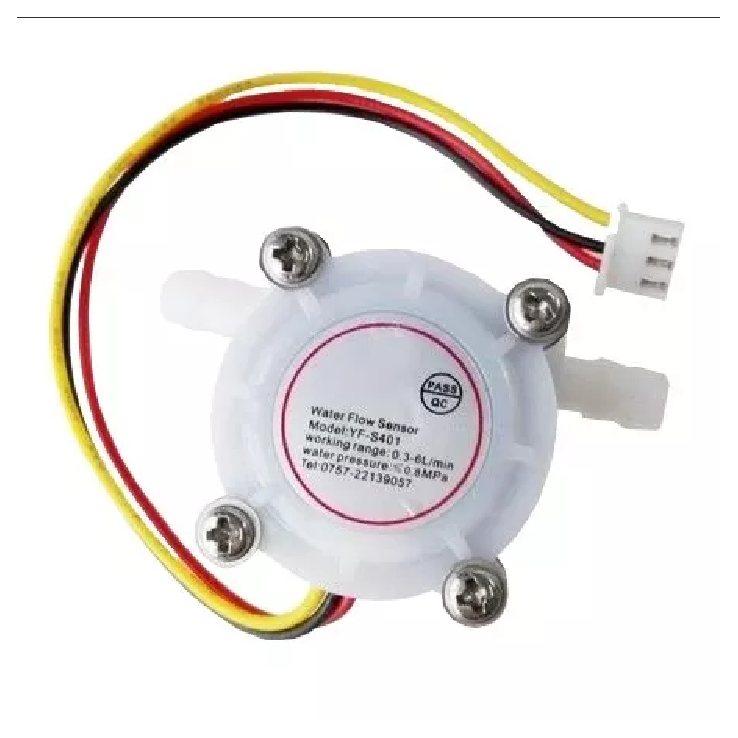
\includegraphics[scale=0.5]{figuras/Figura6.eps}
	\caption{Sensor de Fluxo para a tubulação}               
\end{figure}
\subsection{Explicação}
Este sensor de fluxo ficará posicionado na tubulação do sistema. Seu principal objetivo é monitorar o fluxo do líquido, a fim de acompanhar o funcionamento da bomba d’água. Este sensor servirá como mais um indicativo caso uma falha aconteça no funcionamento da bomba, já que os valores retornados pelo sensor serão fora do esperado, dando pistas sobre qual o possível problema. A escolha deste modelo de sensor de fluxo em específico, se deve a sua ampla utilização no mercado, a sua compatibilidade com diversos microcontroladores existentes, como também suas características, sendo as mais importantes: fluxo de até 6L/min , temperatura de até 80ºC e pressão máxima de até 8 bar. \\
Outro fator importante para a escolha foi a compatibilidade das dimensões do sensor com as dimensões da tubulação, pois um sensor com dimensões diferentes iria requerer o uso de adaptadores para fazer a conexão, o que poderia gerar divergências nas medidas realizadas pelo sensor.\\
Considerando as necessidades apontadas e as características apresentadas pelo sensor, conclui-se que a escolha foi adequada para cumprir satisfatoriamente a função que lhe será imposta.\\
\begin{itemize}
	\item \textbf{Sensor de Nível para o reservatório:}
	\begin{itemize}
		\item \textbf{Nome:} Sensor de Nível de Água com Boia Horizontal;
		\item \textbf{Descrição:} Sensor utilizado para monitorar nível de reservatórios, funcionando como chave magnética nas posições on/off, detectando a presença do líquido no recipiente de acordo com a posição da chave.
		\item \textbf{Tensão de chaveamento (máxima):} 100V DC; 
		\item \textbf{Corrente de chaveamento (máxima):} 0,5A; 
		\item \textbf{Tensão do contato aberto (máxima) :} 220V DC;
		\item \textbf{Resistência Contato (máxima):} 100M Ohms; 
		\item \textbf{Temperatura de operação:} -10 até $+85^oC$;
		\item \textbf{Dimensões:}
		\begin{itemize}
			\item \textbf{Extensão do fio:} 35cm;
			\item \textbf{Diâmetro:} 17mm;
			\item \textbf{Comprimento total:} 82mm;
		\end{itemize}
		
		\item \textbf{Preço:} R\$ 24,90.
		\item \textbf{Observação:} Necessário uso de relé para comunicação com o microcontrolador.
		
	\end{itemize}
\end{itemize}
\begin{figure}[!htb]                   
	\centering                          
	\includegraphics[scale=0.3]{figuras/Figura_7.eps}
	\caption{Sensor de Nível para o reservatório}               
\end{figure}
\subsection{Explicação}
A escolha por este sensor é semelhante à escolha do sensor de fluxo. Considerando o local onde será instalado, suas dimensões se adequam às dimensões do reservatório escolhido para guardar o líquido de arrefecimento, além de possuir compatibilidade com Arduino, PIC, ARM, AVR, dentre outras plataformas de prototipagem. Seu preço, de R\$ 24,90 não é o mais barato dentre as boias vendidas pela empresa, entretanto, as características mostradas acima resultam em um excelente custo-benefício.\\
Cabe ressaltar que o uso de um sensor de nível para o reservatório é imprescindível, pois caso ocorra um vazamento, a leitura de dados indicará um problema, visto que se trata de um sistema fechado. Desta forma, este problema poderá ser solucionado antes que erros mais graves aconteçam, afetando o funcionamento do sistema e consequentemente do sensor de pressão da Kistler.\\
\section{Amplificação de sinais}
A parte de amplificação de sinais é baseada na comunicação entre os sensores e o dispositivo NI 6320, que é uma placa de recolhimento de dados que utiliza o software LabVIEW para análise de dados. Entretanto, tendo em vista que a alguns sensores possuem saída na faixa de miliVolts e a partir dos parâmetros definidos pelo grupo de Processamento de Sinais, para a leitura é necessário um sinal com tensão mínima de entrada que varia entre 0.2 a 10 Volts. Portanto, é necessário um circuito amplificador de sinal entre o sensor e a placa, aumentando proporcionalmente o sinal de saída do sensor, para que a placa possa realizar uma leitura correta dos valores medidos pelo sensor.
\begin{figure}[!htb]                   
	\centering                          
	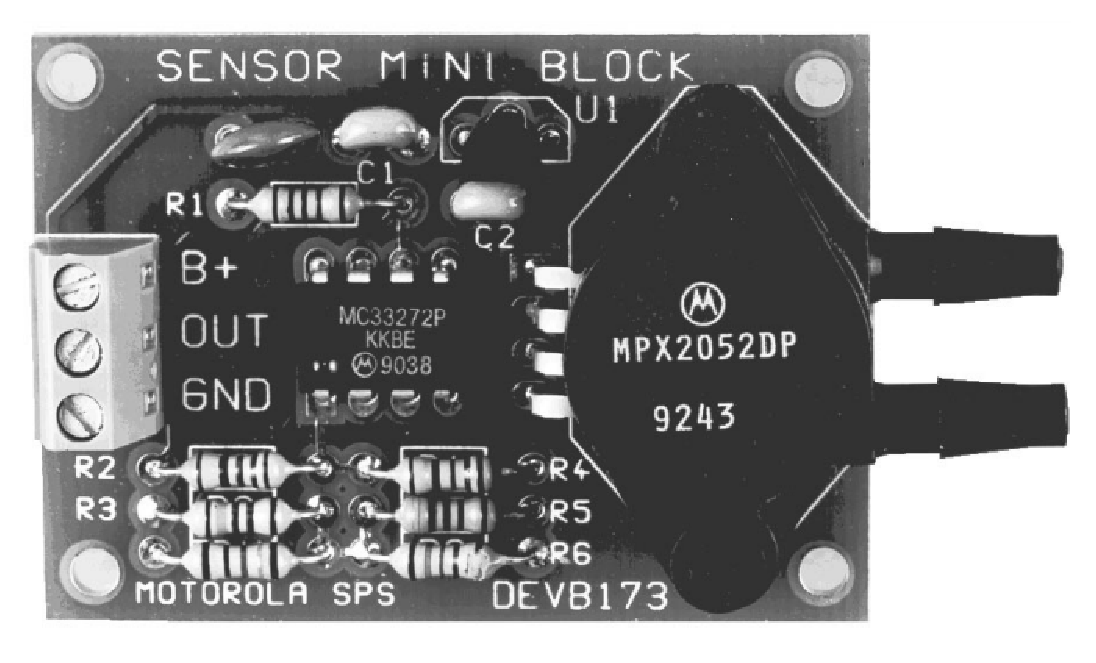
\includegraphics[scale=0.3]{figuras/Figura_8.eps}
	\caption{Circuito Amplificador}               
\end{figure}
\section{Análise de Dados}
Como descrito anteriormente, a análise será feita a partir da placa NI 6320, que utilizará o software LabView para fazer a análise dos dados. Sendo assim, a parte que mais interessa para o controle do sistema, é o retorno dos dados analisados para o microcontrolador, onde de acordo com a análise, o sistema de controle executará uma ação de resposta para estabilizar o sistema.
\section{Transferência de Dados}
A parte de transferência de dados é definida como a parte de comunicação entre a placa e o microcontrolador. Nessa parte, a comunicação será feita de forma paralela, onde a placa enviará os dados para um computador e o computador enviará os dados para o microcontrolador de forma serial por meio de um conector USB.
\section{Controle de Resposta:}
A parte de controle de resposta, corresponde a parte em que o microcontrolador, após receber os dados analisados, executa um comando de resposta de acordo com os dados recebidos. Onde nesse comando será feito o controle de parâmetros como: potência das bombas d'água, velocidade de rotação das ventoinhas e válvulas de controle de fluxo.
Considerando esses fatores, será necessário a utilização de um microcontrolador, e 3 módulos relé para a montagem do sistema de controle.

\subsection{Placa de Processamento}
O sistema terá como placa de processamento a terceira revisão do Arduino Uno (Arduino Rev3), que é uma das placas mais comuns no mercado. A seguir encontram-se as características mais relevantes sobre a placa, para o escopo do projeto:
\begin{itemize}
	\item \textbf{Microcontrolador:} ATmega328
	\item \textbf{Tensão de operação:} 5V
	\item \textbf{Tensão de alimentação recomendada:} 7-12V
	\item \textbf{Tensão máxima suportada:} 20 V (pode causar danos à placa)
	\item \textbf{Entradas digitais:} 14, das quais 6 oferecem entrada PWM (Pulse-Width Modulation)
	\item \textbf{Entradas analógicas:} 6
	\item \textbf{Corrente DC por entrada digital:} 40mA
	\item \textbf{Memória Flash:} 32 KB
	\item \textbf{Memória SRAM:} 2 KB
	\item \textbf{Clock:} 16 MHz
	\item \textbf{Preço:} R\$ 47,90
	
\end{itemize}
\begin{figure}[!htb]                   
	\centering                          
	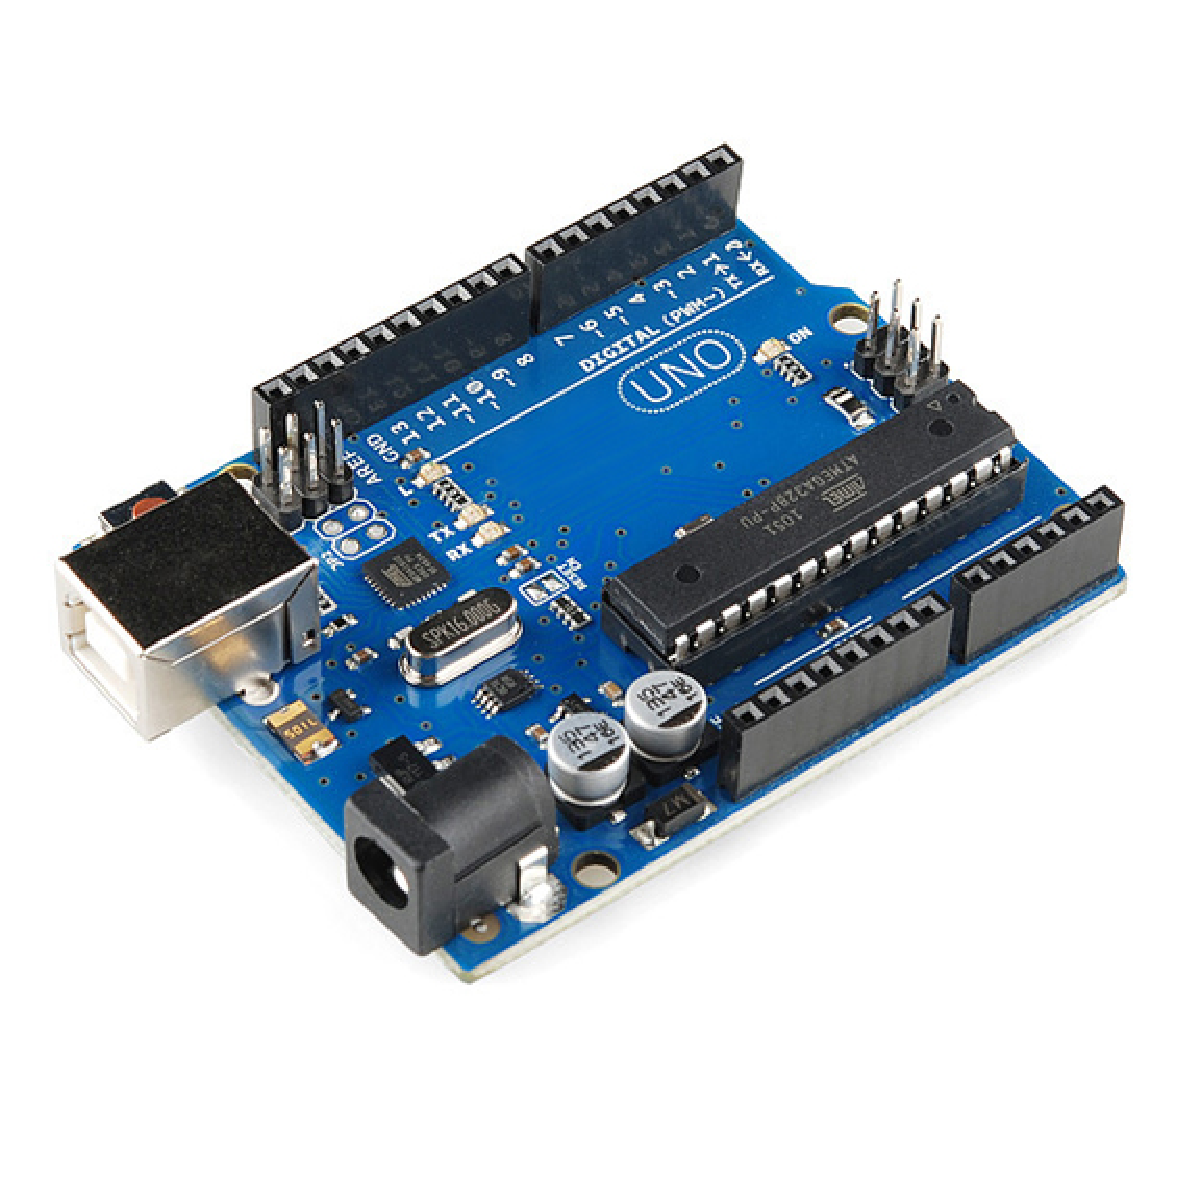
\includegraphics[scale=0.3]{figuras/Figura_9.eps}
	\caption{Arduino Uno}               
\end{figure}
\subsection{Explicação}
A utilização dessa placa de processamento se deve ao fato do seu amplo uso em projetos de controle, tendo uma grande quantidade de bibliotecas, artigos, documentos, funções e informações que auxiliam bastante na construção do projeto. Considerando também suas características apresentadas, outro fator que torna vantajoso a sua utilização é grande quantidade de módulos e shields que funcionam de forma paralela complementando a utilização da placa, aumentando assim suas funcionalidades. \\
E será com o auxílio de módulos que poderá ser realizado o controle dos componentes do sistema de resfriamento, de acordo com a condição que o sistema se encontra no momento. Dessa forma, a escolha da placa se mostra adequada para a situação.\\
\begin{itemize}
	\item \textbf{Módulo Relé para as Bombas d'água:}
	\begin{itemize}
		\item \textbf{Nome:} Módulo Relé 5V 10A 2 Canais com Optoacoplador;
		\item \textbf{Modelo}: SRD-05VDC-SL-C;
		\item \textbf{Tensão de operação:} 5VDC;
		\item Permite controlar cargas de 220V AC;
		\item \textbf{Corrente típica de operação:} 15~20mA;
		\item LED indicador de status;
		\item \textbf{Pinagem:} Normal Aberto, Normal Fechado e Comum;
		\item \textbf{Tensão de saída:} (30 VDC a 10A) ou (250VAC a 10A);
		\item \textbf{Tempo de resposta:} entre 5 e 10 ms;
		\item \textbf{Preço:} R\$12,90.
	\end{itemize} 
\end{itemize}
\begin{figure}[!htb]                   
	\centering                          
	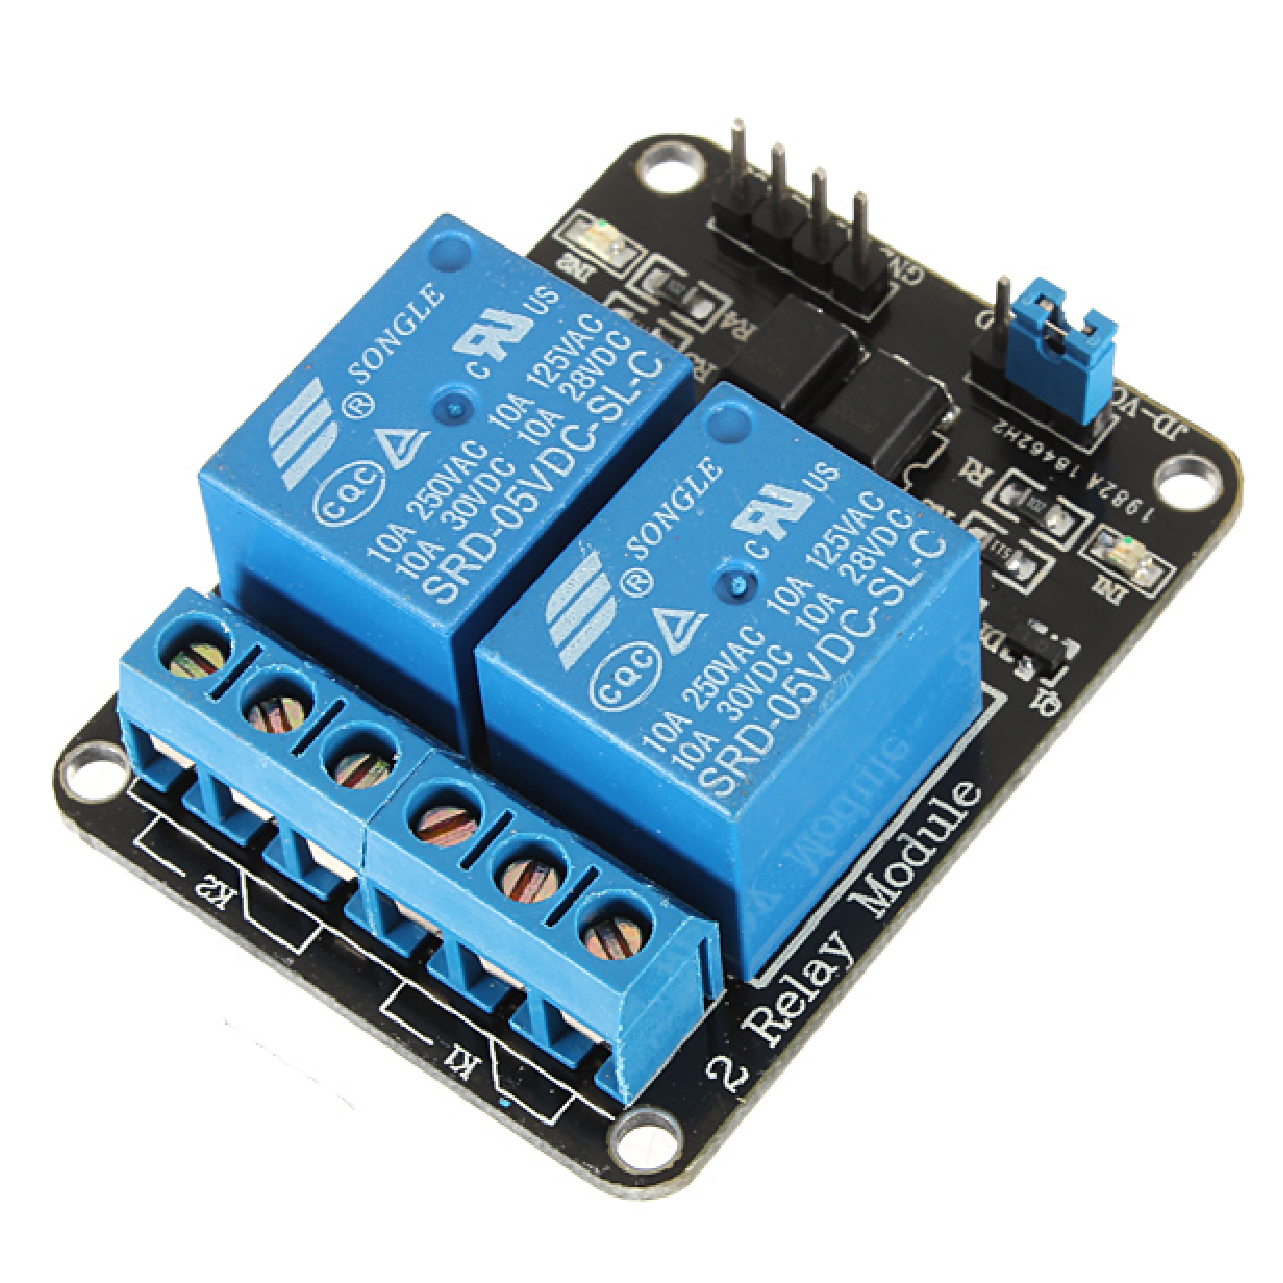
\includegraphics[scale=0.3]{figuras/Figura_10.eps}
	\caption{Módulo Relé}               
\end{figure}	
\subsection{Explicação}
Os módulos relé funcionam como uma chave magnética, onde o sinal digital que vem do microcontrolador que definirá o estado no qual a chave estará. Por se tratar de uma bobina controlada, o módulo relé consegue controlar cargas que exigem uma potência maior que o microcontrolador sozinho poderia fornecer. A utilização desse módulo é explicada, visto que será necessário controlar duas bombas d'água, sendo uma principal e a outra como redundância. Sendo assim, a utilização de um módulo com dois canais se tornou adequada, para uma maior organização na montagem do sistema.\\
\begin{itemize}
	\item \textbf{Módulo Relé para ventoinhas e válvulas hidráulicas:}
	\begin{itemize}
		\item \textbf{Nome:} Módulo Relé 5V 10A 4 Canais com Optoacoplador
		\item \textbf{Modelo:} SRD-05VDC-SL-C 
		\item \textbf{Tensão de operação:} 5VDC
		\item Permite controlar cargas de 220V AC
		\item \textbf{Corrente típica de operação:} 15~20mA
		\item LED indicador de status
		\item \textbf{Pinagem:} Normal Aberto, Normal Fechado e Comum
		\item \textbf{Tensão de saída:} (30 VDC a 10A) ou (250VAC a 10A)
		\item \textbf{Tempo de resposta:} entre 5 e 10 ms
		\item \textbf{Preço:} R\$24,90
	\end{itemize}
	
	
\end{itemize}

\begin{figure}[!htb]                   
	\centering                          
	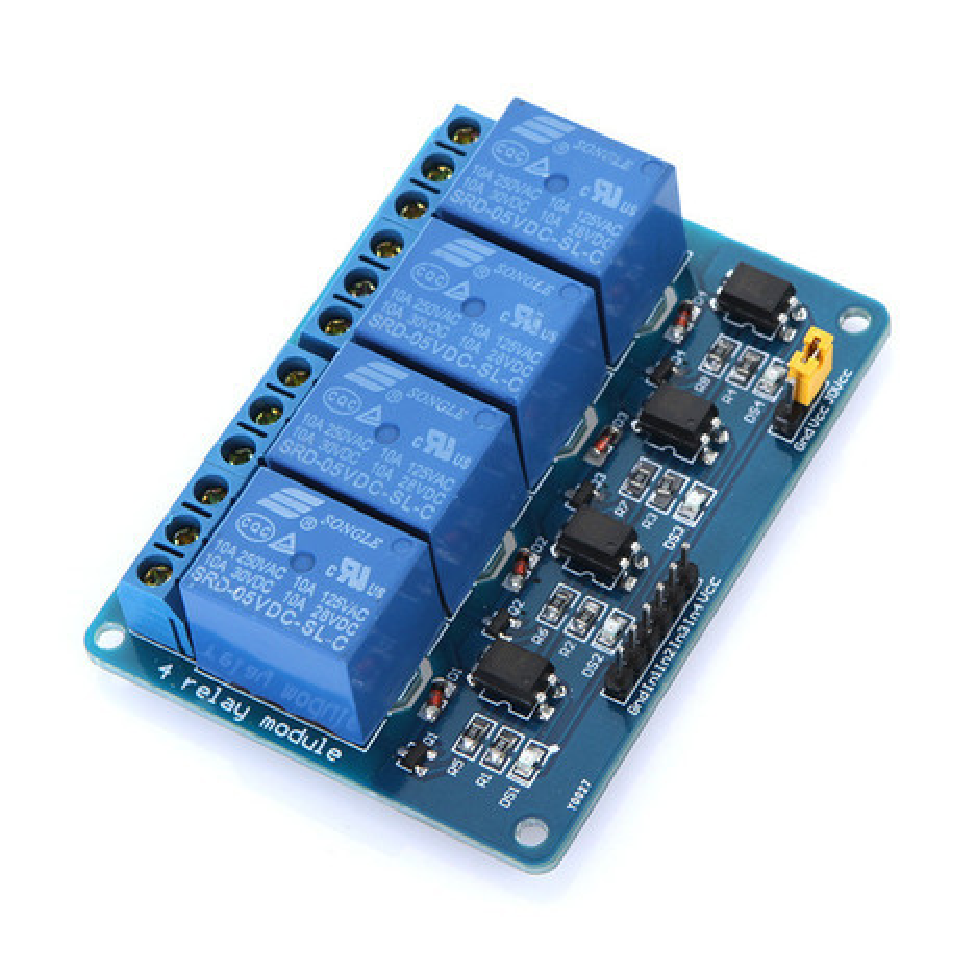
\includegraphics[scale=0.4]{figuras/Figura_11.eps}
	\caption{Módulo Relé para ventoinhas e válvulas hidráulicas}               
\end{figure}
\subsection{Explicação}
Será necessário a utilização de dois módulos desse modelo, visto que um controlará 4 ventoinhas, e o outro controlará duas válvulas hidráulicas, cada uma com dois servos motores. Sendo assim, considerando a utilização e a organização do sistema, a escolha torna-se adequada e prudente.\\
\section{Orçamento}
Na tabela a seguir, estão especificados as quantidades e o preço unitário de cada componente especificado, onde o motivo de duplicata é devido ao fato de se ter um sistema de redundância embutido no sistema, para caso ocorra alguma falha ou emergência. Sendo assim, considerando todos os componentes no que se diz respeito a parte de monitoramento e controle do sistema, o preço final do projeto ficou orçado em R\$ 634,90, sendo considerado apenas o custo com os componentes.
\section{Riscos}

\begin{table}[!htb]
	\centering
	\begin{tabular}{|p{1.5em}|p{4.2em}|p{7em}|p{6.3em}|p{6em}|p{3.8em}|p{4.2em}|}
		\toprule
		\textbf{ID} & \textbf{Risco} & \textbf{Tipo do Risco} & \textbf{Descrição} & \textbf{Descrição do Impacto} & \textbf{Impacto} & \textbf{Probabi- lidade} \\
		\midrule
		\rowcolor[rgb]{ .851,  .851,  .851} R01   & Equipe Grande & \textcolor[rgb]{ .141,  .161,  .18}{Gerenciamento de Projetos} & Equipe possui membros em excesso & Atrapalha o planejamento ocasionando atrasos no projeto & Alto  & Alta \\
		\midrule
		R02   & Falha na comunicação & \textcolor[rgb]{ .141,  .161,  .18}{Gerenciamento de Projetos} & Integrantes não se comunicam devidamente & Ocasiona definições insatisfatórias e má integração do grupo & Alto  & Média \\
		\midrule
		\rowcolor[rgb]{ .851,  .851,  .851} R03   & Falta de integrantes engajados no projeto & \textcolor[rgb]{ .141,  .161,  .18}{Gerenciamento de Projetos} & Desinteresse de parte da equipe & Atrapalha no cumprimento de prazos e na busca por soluções efetivas & Alto  & Alta \\
		\midrule
		R04   & Impossibi- lidade de reuniões presenciais & \textcolor[rgb]{ .141,  .161,  .18}{Gerenciamento de Projetos} & Dificuldade de combinar horários de todos os integrantes do grupo & Atrapalha no desenvolvimento, discussões e definições do projeto & Alta  & Baixa \\
		\midrule
		\rowcolor[rgb]{ .851,  .851,  .851} R05   & Falha no sensor de nível no reservatório & \textcolor[rgb]{ .141,  .161,  .18}{Técnico} & Medição com valores muito diferentes do esperado ou a não medição & Causa uma estimativa errônea sobre o volume de água no reservatório & Médio & Muito Baixa \\
		\midrule
		R06   & Falha no sensor de temperatura do reservatório(ST1) & \textcolor[rgb]{ .141,  .161,  .18}{Técnico} & Medição com valores muito diferentes do esperado ou a não medição & Ocasiona uma resposta errônea do sistema de arrefecimento & Médio &  Muito Baixa \\
		\bottomrule
	\end{tabular}
	\caption{Tabela de riscos}
\end{table}

\newpage

